\section{Dynamical systems}

A system can be defined as any transformation between an input signal and output signal. Denoting the system by $\mathcal{S}_0$, and the input/output signals by $u_0$ and $y_0$ respectively, we will leave the nature of these terms unspecified for the moment. In order to interact with the system, and in particular take measurements of the input and output quantities, the presence of measurement noises should also be acknowledged. Thus, a complete picture of the system and its measured signals is shown in the block diagram of Figure \ref{fig:SysIDoverview}, where $v_u$ and $v_y$ denote noise signals which corrupt the measurement of $u_0$ and $y_0$ respectively, with $u$ and $y$ representing the noisy measured signals.

\begin{figure}[h]
\centering
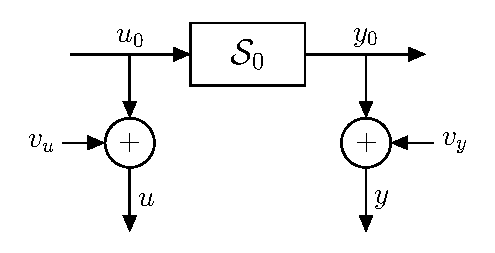
\includegraphics[width=0.5\textwidth]{Chapter2_SysIDandControl/SysIDoverview.pdf}
\caption{Generic block diagram of a system with input and output measurement noise}
\label{fig:SysIDoverview}
\end{figure}

Before considering identification or control, the nature of the system under study and its associated signals must be further clarified. There are a number of system characterizations which must be determined (or chosen), which are listed and defined below:

\begin{enumerate}
\item \textbf{Dynamic/Static:} A system which is dynamic has the property that the current output, denoted by $y(t)$, depends not only on the current input, $u(t)$, but also on past values of the input and/or output, $u(t-\tau)$ and $y(t-\tau)$ for $\tau>0$. It is equivalent to say that dynamic systems possess memory. Conversely, a static system is a memory-less system, where the current output is dependent only on the current input.
\item \textbf{Linear/Nonlinear:} A system is defined as linear if it satisfies the properties of homogeneity and additivity, i.e. the following condition is true:
\begin{align}
\mathcal{S}_0: u_1 \rightarrow y_1 \text{ and } \mathcal{S}_0: u_2 \rightarrow y_2 &\implies \mathcal{S}_0: \alpha u_1+ \beta u_2 \rightarrow \alpha y_1+ \beta y_2 \; \; \forall \alpha, \beta.
\end{align}
If this condition is not satisfied in general, the system is nonlinear.
\item \textbf{Time-invariant/Time-varying:} A time-invariant system does not change the nature of its input-output transformation over time, while for time-varying systems, the time at which a given input is applied can change the resulting output. 
\item \textbf{Discrete-time/Continuous-time:} A system which is discrete-time performs transformations using sampled input and output signals. This means that the signals $u(t)$ and $y(t)$ are defined only for specific values of $t$. When the samples are regular (evenly spaced), the argument $t$ is typically restricted to integer values to represent the sample number. Continuous-time systems, as the name suggests, consider input signals which are continuous functions and produce a corresponding continuous output signal. It is worthwhile to note that while virtually all physical systems are continuous in nature, the discrete-time framework is useful in our digital world where measurements are taken and stored as discrete samples. 
\item \textbf{SISO/MIMO:} A single-input-single-output (SISO) system possesses scalar input and output signals. Conversely, a multiple-input-multiple-output (MIMO) system may have multiple signals at the input and output ports. This means that the signals $u(t)$ and $y(t)$ at any instance of $t$ are \emph{vectors} containing multiple scalar components.
\end{enumerate}

Many of the above characterizations should be considered as mathematical approximations, rather than concrete physical properties of the system. For example, it would be fair to say that no real system is truly linear, however there are many systems for which a linear model is satisfactory in capturing the important dynamic behaviour for prediction or control purposes \cite{Pintelon2012}. Indeed, the entire pursuit of prescribing a mathematical model to a real process should be considered an abstraction from reality, since an exact description is never attainable. This philosophical perspective is eloquently presented in \cite{Ljung1987}:
\begin{quote}
``In a sense, there is an impenetrable but transparent screen between our world of mathematical descriptions and the real world. We can look through this window and compare certain aspects of the physical system with its mathematical description, but we can never establish an exact connection between them.'' \hfill (Lennart Ljung)
\end{quote} 

Nevertheless, all systems must be characterized in a mathematical sense prior to modeling. In this thesis, we will focus on SISO systems which are well approximated by a discrete-time, dynamic, nonlinear, time-invariant description.

\section{The identification process}

When it comes to the identification of a dynamical system from experimental data, there are a number of distinct steps in the process. Naturally, much of the attention in system identification literature is focussed on estimation algorithms, and how to transform the measured data into an accurate system model. However, before the estimation stage there are other considerations to be made. These considerations include the experimental procedure which should be designed in order to obtain informative data from the system, the model structure which must be chosen for estimation, and a metric which should be constructed to quantify the performance of candidate models during estimation. Even after a model estimate has been obtained, there is further work in validating the model on separate data to ensure it meets specifications for the intended use.

An overview of the full identification process is depicted in Figure \ref{fig:IdentProcess}. Note that many of the stages can be informed by prior knowledge of the system, as well as previous unsuccessful estimation attempts. The latter point highlights the iterative nature of system identification. It can be difficult to choose the experimental conditions, model class, etc. in an optimal way without yet having a mathematical system description, however those initial attempts which do not meet specifications can provide information for revising and improving the process. 

\begin{figure}[h]
\centering
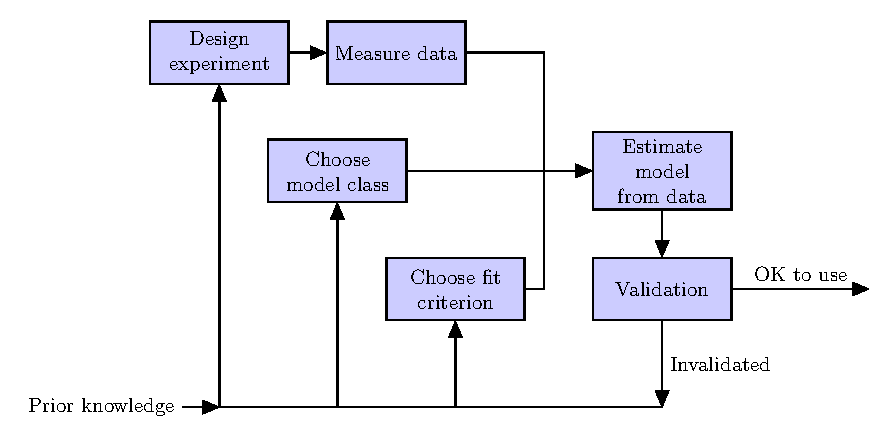
\includegraphics[width=0.9\textwidth]{Chapter2_SysIDandControl/IdentificationProcess.pdf}
\caption{An overview of the identification process}
\label{fig:IdentProcess}
\end{figure}

Background will be provided in the following subsections for each stage in the identification process. These sections will also provide some context regarding each stage in terms of this thesis.

\subsection{Experiment design} 

Broadly speaking, the objective when designing an identification experiment is to ensure that the measured data provides maximal information with respect to the intended use of the system model \cite{Gevers1986}. The experiment design should cater to any practical constraints which are present, and consider factors such as experiment duration, presence of stabilizing feedback, and most importantly, the nature of the excitation signal. Optimal input design has itself become a rich sub-field, which considers how best to choose the class of signal used for excitation, as well as its power spectrum and range \cite{Bombois2006}, \cite{Hildebrand2007}.

Experiment design is not a crucial element of this thesis. Several signal classes are used for excitation, including Gaussian white noise, pseudo-random binary sequence (PRBS), and random phase multisine. White noise and PRBS have an approximately flat power spectrum across the entire frequency band, while multisines allow precise control over the power contained at each frequency \cite{Schoukens2016}, being explicitly constructed from the sinusoid summation: 
\begin{equation}
u_0(t) = A_0 + \sum_{i=1}^{F} A_i \text{cos}(2 \pi i f_0 t + \phi_i),
\end{equation}
where $A_0$ gives the constant offset, $f_0$ is the fundamental frequency (in Hz), $F$ is the maximum harmonic excited, and $\phi_i$ are randomly selected phase shifts.

\subsection{Choosing a model class}

A plethora of model classes exist for describing dynamical systems, and a selection here has consequences for the estimation methods which can be used as well as the suitability of the estimated model for its intended use. The first choice which should be made is whether to use a parametric or nonparametric representation. While parametric models have a fixed and finite number of parameters, nonparametric models are characterized by a parameter set which is infinite in theory and in practice can grow indefinitely with increasing data length. Another crucial question is whether to construct a model in the time or frequency domain, i.e. whether to express the input to output transformation in terms of time domain or frequency domain signals.

For discrete linear systems, popular model classes include the parametric ARMAX, Box-Jenkins and state space structures, as well as the nonparametric impulse response model and its frequency domain equivalent, the frequency response function (FRF). For nonlinear systems, as discussed in Chapter \ref{chap:1}, there are a number of representations available. NARMAX and block-oriented models can be fully or partially parametric, while the Volterra series and its related expansions are nonparametric. The Volterra series also has a frequency domain equivalent formulation comprised of GFRFs. This thesis assumes a preference for nonparametric modeling, and deals with Volterra series estimation in both time and frequency domain. Other nonlinear model classes, e.g. block-oriented structures, are sometimes used to construct a simulated `true system' on which identification is performed.

When a model class has been selected, it defines a set, $\mathcal{M}$, of all possible models for the system. The set is defined as
\begin{equation}
\mathcal{M} := \{ \mathcal{S}(\theta) | \theta \in \Theta \subset \mathbb{R}^n \}
\end{equation}
where $\theta \in \mathbb{R}^n$ is a vector of parameters completely describing the model, $\Theta$ is the vector space of all possible parameter vectors, and $\mathcal{S}(\theta)$ is the parameterized system model.


\subsection{Choosing the fit criterion}

Once experimental data has been collected and a model class chosen for a system, a metric $V(\theta)$ is defined in order to differentiate the performance of model candidates in the estimation stage. This metric will be labelled the `fit criterion', which for any given $\theta$ assigns a numeric value representing how well the corresponding model fits the observed experimental data. 

The fit criterion should be chosen based on the context in which the model will be used, but care must be taken since this choice will also have implications for computational complexity in the estimation phase. Typically, the criterion $V(\theta)$ is based on some measure of distance between the measured output and the model output predicted using $\mathcal{S}(\theta)$. Alternatively (and sometimes equivalently), $V(\theta)$ can be formulated as a statistical likelihood function which provides the likelihood of seeing the observed data given a model parameterized by $\theta$ and some assumed measurement noise distributions. 

The estimation methods developed in this thesis use fit criteria which can be framed both in terms of a distance measure and a statistical function, with the relationship between the two criteria discussed in Section \ref{sec:ReLS_Chap2}.

\subsection{Model estimation}

The specific details of model estimation will depend heavily on the model structure and fit criterion which have been chosen in the previous stages. In the most general case, model estimation can be framed simply as the optimization of a criterion $V(\theta)$ over the allowable space $\Theta$. For example, if the criterion is a distance measure between the measured and predicted outputs, our model can be defined by the minimization problem:
\begin{equation}
\hat{\theta} = \text{arg } \underset{\theta}{\text{min}} \; V(\theta).
\end{equation}

Depending on the complexity of the model and fit criterion, solving the optimization problem can be as simple as an analytic solution. Conversely, $V(\theta)$ may be highly non-convex, requiring techniques that can efficiently locate a global optimum. The estimation methods in this thesis will feature minimization problems of the latter type, and the efficiency of finding solutions is addressed in Chapter \ref{chap:4}.

\subsection{Validation}

After obtaining a model estimate, it is important to test the model's prediction accuracy on a new set of experimental data, known as validation data, which is uncorrelated with the data used for estimation. This allows a user to assess whether the model meets the specifications for its intended purpose, and will also detect problems like overfitting, where some of the model parameters are inadvertently used to capture the noise in the estimation data rather than the underlying process.   

\section{The impulse response model}

The impulse response model is a foundation stone of linear systems theory. For a discrete-time SISO system, it is defined as the output response to a unit impulse applied at sample time $t=0$, i.e. $u(t) = \delta(t)$ where $\delta(t)$ denotes the discrete-time unit impulse function,
\begin{equation}
\delta(t) = \begin{cases} 1 & \text{for } t = 0 \\
0 & \text{for } t \neq 0 \end{cases}
\end{equation}

This impulse response is denoted by $h(t)$, which can be infinite in length. The infinite impulse then forms a unique description for any linear system, since the system response to any arbitrary input is just a convolution of the input with the impulse response,
\begin{equation}
\label{eq:IIRdefn}
y(t) = \sum_{\tau=-\infty}^{\infty} h(\tau) u(t-\tau) = h(t) * u(t),
\end{equation}
where $*$ is the convolution operator. It is clear that $h(t)$ represents a nonparametric model structure for linear systems, which will be denoted the infinite impulse response (IIR) model.

Models of infinite dimension are not useful in a practical setting, however there are some generic properties of a linear impulse response which are independent of the generating system, and these properties can be exploited to produce a finite-parameter model. First, we impose an assumption of causality (no system can predict the future), such that $h(t) = 0$ for $t<0$. Thus, the negative tail of the impulse can be disregarded. We will also restrict our scope to the set of stable linear systems, which brings an additional implication that the impulse response tends to 0 over time:
\begin{equation}
h(t) \xrightarrow{\: t \to \infty \:} 0.
\end{equation} 

Under these conditions, it follows that any impulse response model can be truncated to a finite length, $t= 0,1,\hdots,n-1$, where $h(n)$ is the first negligible component as dictated by some user-specified threshold. The truncation length $n$, will be referred to as the `effective memory length' of the system. The truncated impulse forms a new nonparametric description which will be denoted the finite impulse response (FIR) model, and written mathematically as, 
\begin{equation}
\label{eq:FIRdefn}
y(t) = \sum_{\tau=0}^{n-1} h(\tau) u(t-\tau).
\end{equation}
Examples of truncated impulse responses are shown in Figure \ref{fig:ImpulseExamples} for arbitrary linear systems. 

\begin{figure}[h]
\centering
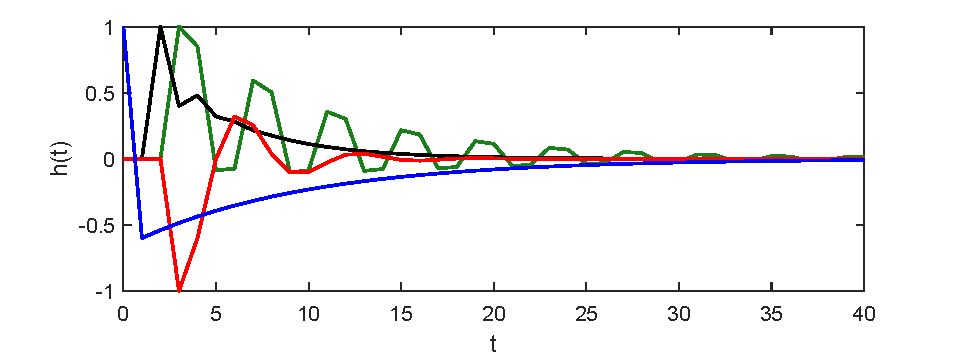
\includegraphics[width = 0.9\textwidth]{Chapter2_SysIDandControl/RandomFIRs}
\caption{Example impulse responses for randomly generated discrete linear filters}
\label{fig:ImpulseExamples}
\end{figure}

\section{Classical estimators}

For the identification of dynamical systems, it is often possible to formulate the estimation problem such that classical estimation techniques can easily be applied. An example of this is when the system model is `linear-in-the-parameters'. Assuming we have some parameter vector $\theta \in \mathbb{R}^{n}$ which is a column vector, a linear-in-the-parameters model has output response at sample $t$ given by:
\begin{equation}
\label{eq:LeastSquares_1row}
y(t) = \phi(t)^T \theta + e(t)
\end{equation}
where $T$ is the vector transpose operator. The $e(t)$ term captures any error between the measured output and model, and $\phi(t) \in \mathbb{R}^{n}$ is known as the regressor vector, which can contain any mixture of past output and input samples depending on the model structure. If we consider the FIR model from (\ref{eq:FIRdefn}), which is linear-in-the-parameters, then (\ref{eq:LeastSquares_1row}) holds with
\begin{align}
\theta &= [h(0) \; h(1) \; \hdots \; h(n-1)]^T, \label{eq:ParameterVector4Impulse} \\
\phi(t) &= [u(t) \; u(t-1) \; \hdots \; u(t-n+1)]^T.
\end{align}

While (\ref{eq:LeastSquares_1row}) explains the output response for a single sample, $t$, the representation can be extended to model an entire output data record. Assuming $N$ samples of input and output data ($t = 0, \hdots, N-1$) are measured from a system, and considering the FIR model (\ref{eq:FIRdefn}), an output vector $Y = [y(n-1) \; y(n) \; \hdots \; y(N-1)]^T$ is constructed and modeled as,
\begin{equation}
\label{eq:LeastSquares_allrows}
Y =  \Phi^T \theta + E
\end{equation}
where $E$ is a vector containing the errors $e(t)$, and $\Phi \in \mathbb{R}^{n \times (N-n+1)}$ is the regressor matrix, given by
\begin{equation}
\Phi = \begin{bmatrix} \phi(n-1) &\phi(n) &\hdots &\phi(N-1) \end{bmatrix}.
\end{equation}

\subsection{The least squares approach}

In order to estimate $\theta$ from (\ref{eq:LeastSquares_allrows}), a fit criterion $V(\theta)$ is required. The least squares (LS) approach employs a sum of squared errors between the model and the measurement as such a criterion. Mathematically, the LS criterion can be expressed as,
\begin{align}
V_{LS}(\theta) &= E^T E \\ 
&= (Y-\Phi^T \theta)^T(Y - \Phi^T \theta) \\
&= \norm{(Y-\Phi^T \theta)}_2^2,
\label{eq:LS_criterion}
\end{align}
where $\norm{\cdot}_2^2$ denotes the squared 2-norm operator. The resulting optimization problem to obtain our estimate $\hat{\theta}$, is given by
\begin{equation}
\hat{\theta} = \text{arg } \underset{\theta}{\text{min}} \; \norm{(Y-\Phi^T \theta)}_2^2,
\label{eq:LS_opt}
\end{equation}
which is easily shown to be a convex problem with the analytic solution,
\begin{equation}
\hat{\theta} = (\Phi \Phi^T)^{-1}(\Phi Y).
\label{eq:LS_analytic}
\end{equation}

For the least squares approach, the interpretation of `error' is quite general. it can represent output measurement noise, or model errors due to a mismatch between the model and true system, or a combination of both. Of course, the true source of these errors will have an effect on the properties of the least squares estimator, however before discussing this, the maximum likelihood estimator will be derived for our linear-in-the-parameters structure.

\subsection{Maximum likelihood estimation}

In maximum likelihood estimation (MLE), our fit criterion is chosen as the likelihood function, $\mathcal{L}(Y;\theta)$, which gives the likelihood of observing the output vector $Y$ given some model structure parameterized by $\theta$. In order to express the likelihood analytically, the system model should have some statistical properties imposed, and in particular for our linear-in-the-parameters representation (\ref{eq:LeastSquares_allrows}), the stochastic behaviour of the error vector $E$ should be defined.

One common assumption for $E$, and the one which will be discussed here, is that $E$ is a vector of independent and identically distributed (i.i.d.) random variables each with a zero mean normal distribution. Observing Figure \ref{fig:SysIDoverview}, this assumption implies that we have Gaussian white measurement noise at the output ($v_y(t) = e(t)$), and no input noise ($v_u = 0$). This produces a stochastic model description for $Y$, i.e.
\begin{equation}
Y \sim \mathcal{N}(\Phi^T \theta,\sigma^2 I),
\end{equation}
where $\sigma^2$ is the variance of the errors in $E$, and $I$ is an identity matrix of appropriate size. An analytic expression for the likelihood, and thus the fit criterion, can be written using the multivariate normal distribution, yielding
\begin{equation}
V_{ML}(\theta) = (2 \pi \sigma^2)^{-\frac{N-n+1}{2}} \text{exp}\bigg( -\frac{1}{2 \sigma^2} \norm{(Y-\Phi^T \theta)}_2^2 \bigg).
\label{eq:ML_criterion}
\end{equation}
The optimization problem for estimating $\theta$ is simply to maximize the likelihood function,
\begin{equation}
\hat{\theta} = \text{arg } \underset{\theta}{\text{max}} \; V_{ML}(\theta).
\label{eq:ML_opt}
\end{equation}

It is trivial to show that under the assumption above on the error, and substituting (\ref{eq:ML_criterion}) into (\ref{eq:ML_opt}), the problem will reduce to (\ref{eq:LS_opt}). Thus the maximum likelihood approach shares the same analytic solution (\ref{eq:LS_analytic}) as the least squares approach for this case. This explains the popularity of the Gaussian measurement noise assumption in MLE, since it produces a familiar analytic solution. However, the estimator performance will degrade if there is significant input measurement noise, or the output noise is a correlated (non-white) sequence. In these circumstances, a more complex stochastic model may be required.

\subsection{Estimator properties}

\begin{defn}[Estimator]
For a model set $\mathcal{M}$, an estimator is an operator which maps the measured data $u$ and $y$ to a parameter vector estimate $\hat{\theta}$. 
\end{defn}
To analyze the properties of an estimator, the philosophical truth that real systems can never be fully described by abstract models will be abandoned out of necessity, and replaced with the pretence that there exists a true \emph{mathematical} description of the system, $\mathcal{S}_0$. Under the further condition that this true system lies within our model set, i.e. $\mathcal{S}_0 \in \mathcal{M}$, the notion of a true parameter vector can be introduced.
\begin{defn}[True parameters]
The true parameter vector, $\theta_0$, is a vector satisfying $\mathcal{S}(\theta_0) = \mathcal{S}_0$.
\end{defn}

Any estimate $\hat{\theta}$ produced by an estimator is a function of input and output measurements obtained from the system, which contain stochastic noise in general. The estimate itself should therefore be treated as a random variable, and it is the statistical properties of this variable which define the performance of the estimation method. There are three properties in particular which, when combined, provide an appreciation of the performance of the estimator. They are the bias, covariance and mean square error (MSE).

\begin{defn}[Bias]
The bias of an estimator is the difference between the expected value of the estimate and the true parameters:
\begin{equation}
\Bias(\hat{\theta}) = \textbf{E}\{ \hat{\theta} \} - \theta_0.
\end{equation}
An unbiased estimator is one for which $\textbf{E}\{ \hat{\theta} \} = \theta_0$.
\end{defn}

\begin{defn}[Covariance]
The covariance of an estimator is its variability or dispersion around the expected value, described by:
\begin{equation}
\Cov(\hat{\theta}) =  \textbf{E} \bigg\{ \big( \hat{\theta} - \textbf{E}\{ \hat{\theta} \} \big) \big( \hat{\theta} - \textbf{E}\{ \hat{\theta} \} \big)^T \bigg\}.
\end{equation}
\end{defn}

\begin{defn}[MSE]
The MSE of an estimator combines the effects of bias and covariance into a total error metric, given by:
\begin{align}
\MSE(\hat{\theta}) &=  \textbf{E} \bigg\{ \big( \hat{\theta} - \theta_0 \big) \big( \hat{\theta} - \theta_0 \big)^T \bigg\} \\
&= \Bias(\hat{\theta}) \Bias(\hat{\theta})^T + \Cov(\hat{\theta}).
\end{align}
\end{defn}

Observing these three properties, it is clear that an accurate estimator should have the lowest possible bias and covariance (in the matrix sense) in order to minimize its MSE. It would seem natural then, to consider only unbiased estimators such that $\text{Bias}(\hat{\theta}) = 0$. Indeed, the LS and MLE estimators, (\ref{eq:LS_opt}) and (\ref{eq:ML_opt}), will be unbiased under the following conditions:
\begin{enumerate}
\item $\mathcal{S}_0 \in \mathcal{M}$
\item No input measurement noise
\item The output error $E$ is any zero mean stochastic process
\end{enumerate}
Note that in the MLE case, the Gaussian i.i.d. noise assumption need not be met to ensure unbiasedness. Covariance, on the other hand, will reduce further under the correct noise distribution. There is a fundamental restriction on how far the covariance can decrease in unbiased estimators, and this is known as the Cramér-Rao lower bound \cite{Pintelon2012}. An unbiased estimator with covariance obtaining the lower bound is called an \emph{efficient} estimator. 

When considering models which require many parameters, such as the nonparametric impulse response, the Cramér-Rao lower bound can present a problem. For example, when the number of samples $N$ used in the estimation is low, or measurement noise is significant, even an efficient estimator will have very high covariance and hence is likely to produce an inaccurate model. In these cases, it can be beneficial to introduce a small bias into the estimator in such a way that the covariance reduces dramatically along with the MSE. Typically, this bias reflects some prior belief on how the parameter vector should behave, and can be introduced by adding an additional penalty to the fit criterion (known as `regularization'), or by adopting a Bayesian estimation approach. These two techniques are intrinsically related and will form the core of all identification methods presented in this thesis.

\section{Regularized least squares and the Bayesian {perspective}}
\label{sec:ReLS_Chap2}

The least squares approach to model estimation is attractive due to its simplicity, with an analytic solution guaranteed for any model structure that is linear-in-the-parameters as long there is enough measurement data available. In practice however, and particularly for nonparametric structures such as the FIR model, estimation using least squares will lead to poor results under many circumstances. The issues relevant to FIR estimation are:
\begin{itemize}
\item The estimator will have large covariance if the number of data points $N$ does not greatly exceed the number of parameters, $n$.
\item The estimator will have large covariance when output measurement noise is significant.
\item The estimation problem will be ill-conditioned if the input excitation is not sufficiently exciting.
\item The estimation problem does not have a unique solution when $N < 2n-1$.  
\end{itemize} 
Observing these issues, it is clear that a long, well designed and relatively noise-free experiment is required to achieve good impulse response estimates, particularly when the impulse has a large effective memory length, $n$. There are many practical identification settings where such ideal experimental conditions are not possible, and consequently will require more advanced estimation techniques. 

As an example, FIR model estimates are obtained for a simulated linear system using least squares on two sets of experimental data, where each experiment has Gaussian excitation $u(t) \sim \mathcal{N}(0,1)$ and Gaussian measurement noise $e(t) \sim \mathcal{N}(0,\sigma^2)$.  The first experiment records $N=2000$ data samples and $\sigma^2$ is chosen such that the Signal-to-Noise Ratio (SNR)\footnote{SNR is defined using the variance ratio: SNR = $\Var [y_0]/\Var [e]$} is 40dB. The second experiment records only $N=200$ samples with a decreased SNR of 20dB. The least squares estimated impulse response for each experiment is plotted in the left half of Figure \ref{fig:ExampleImpulseEsts}, along with the true system, showing the performance degradation that comes with small data lengths and high noise levels. The right half of Figure \ref{fig:ExampleImpulseEsts} plots \emph{regularized} estimates for the same experiments, which are seen to be far less sensitive to decreases in data length and SNR. The mathematical techniques for performing regularized FIR estimation will now be discussed.

\begin{figure}[h]
\centering
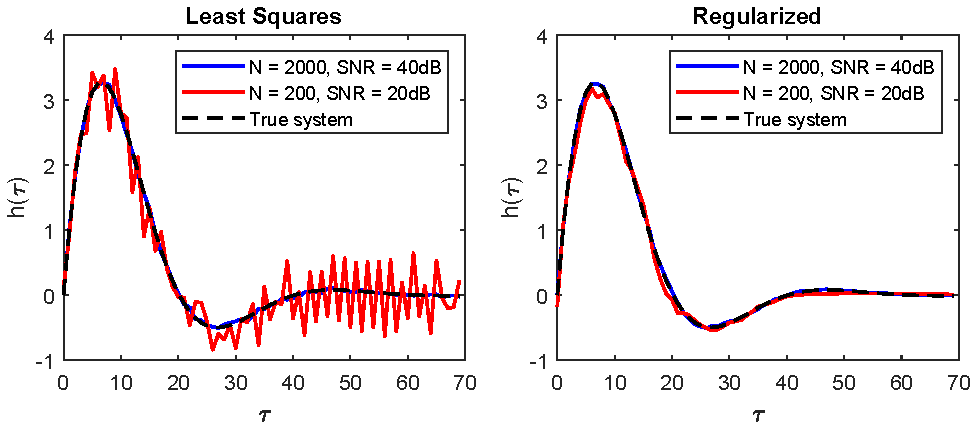
\includegraphics[width = 0.98\textwidth]{Chapter2_SysIDandControl/LS_example2}
\caption{Least squares (left) and regularized (right) FIR estimates for an example linear system using different data lengths and SNRs}
\label{fig:ExampleImpulseEsts}
\end{figure}

\subsection{Regularization penalty options}

In its most general form, regularization can be described as the inclusion of an additional term in the fit criterion of an estimator. The regularized least squares (ReLS) criterion is then given by,
\begin{equation}
V_{ReLS}(\theta) = \norm{(Y-\Phi^T \theta)}_2^2 + T(\theta),
\end{equation} 
where $T(\theta)$ is an additional penalty term acting directly on the parameter vector. Such an addition can be used to impose certain expected behaviours on the estimated parameter vector, thereby reducing the effect of noisy measurements and improving the estimation accuracy. In ill-posed estimation problems, the added penalty can also improve conditioning.

Various forms have been proposed for $T$, starting with the early results of Tikhonov \cite{Tikhonov1963}, for which the term `Tikhonov regularization' was coined. The penalty for this type of regularization takes the general form:
\begin{equation}
T(\theta) = \norm{\Gamma \theta}_2^2,
\label{eq:TikhonovPenalty}
\end{equation}  
where $\Gamma$ is a Tikhonov matrix chosen to impose certain parameter behaviours. When the Tikhonov matrix is chosen as a multiple of the identity matrix, i.e.
\begin{equation}
T(\theta) = \gamma \norm{\theta}_2^2,
\end{equation}
for some $\gamma \in \mathbb{R}^+$, then the regularization method is known within the statistics community by the term `ridge regression' \cite{Hoerl1970}. This scheme is particularly useful for parameter vectors which are expected to be sparse, since parameters are heavily penalized for being too far from zero. If the parameters in $\theta$ have different physical units, appropriate pre-scaling should be applied.   

A more recent proposal for regularized estimation of sparse parameter vectors is the lasso (Least Absolute Shrinkage and Selection Operator) algorithm \cite{Tibshirani1996}, which replaces the 2-norm penalty with a 1-norm, giving
\begin{equation}
T(\theta) = \gamma \norm{\theta}_1.
\end{equation}
The lasso approach has been shown to exhibit some nice properties with respect to capturing the set of zero elements in the true parameter vector, $\theta_0$ \cite{Tropp2006}. 

Yet another similar technique is nuclear norm regularization \cite{Fazel2001}, \cite{Mohan2010}, which uses penalty term
\begin{equation}
T(\theta) = \gamma \norm{H(\theta)}_*,
\end{equation}
with $H(\theta)$ denoting the Hankel matrix of $\theta$, and $\norm{\cdot}_*$ being the nuclear norm operator, defined as the sum of singular values of its matrix argument. The nuclear norm has been shown to be a convex approximation of the matrix rank function \cite{Fazel2001}, and for $\theta$ given by an impulse response model (as in (\ref{eq:ParameterVector4Impulse})), penalizing the Hankel matrix rank is equivalent to penalizing the order (i.e. complexity) of the linear system.

\subsection{The quadratic penalty}

One penalty term in particular has garnered a significant amount of attention in recent decades, first in the machine learning field for function estimation \cite{Rasmussen2006}, before being introduced to the system identification community as a method of low covariance impulse response estimation \cite{Pillonetto2010}. The penalty is quadratic in nature, having the form,
\begin{equation}
T(\theta) = \gamma \theta^T P^{-1} \theta.
\label{eq:QuadraticPenaltyT}
\end{equation}
Comparison with (\ref{eq:TikhonovPenalty}) reveals this term to be just a special case of Tikhonov regularization, where $\gamma P^{-1} = \Gamma^T \Gamma$. 

The total regularized estimation problem with the quadratic penalty (\ref{eq:QuadraticPenaltyT}) can be stated as
\begin{equation}
\hat{\theta} = \text{arg } \underset{\theta}{\text{min}} \norm{(Y-\Phi^T \theta)}_2^2 + \gamma \theta^T P^{-1} \theta,
\label{eq:Estimator_QuadraticPenalty}
\end{equation} 
which is a convex problem with an analytic solution,
\begin{equation}
\hat{\theta} = (P \Phi \Phi^T + \gamma I)^{-1} P \Phi Y.
\label{eq:QuadraticPenalty_analyticsolution}
\end{equation} 
The terms $\gamma$ and $P$ are tunable, with $P$ enforcing certain behaviours in the estimated parameter vector and $\gamma$ scaling the effect of the regularization, much like generic Tikhonov regularization. It is the specific techniques for designing and tuning these terms, however, which has recently received an explosion of interest \cite{Pillonetto2014}. To understand how these techniques emerged, it is important to first look at the MSE property of our regularized estimator (\ref{eq:QuadraticPenalty_analyticsolution}).

It will be assumed that we have the linear-in-the-parameters model (\ref{eq:LeastSquares_allrows}) with true parameter vector $\theta_0$, and i.i.d. errors such that $\mathbf{E} \{ EE^T \} = \sigma^2 I$. Under these conditions, it can be shown that the MSE of (\ref{eq:QuadraticPenalty_analyticsolution}) is minimized (in the matrix sense) by the following choices \cite{Chen2012}:
\begin{align}
\gamma &= \sigma^2, \\
P &= \theta_0 \theta_0^T. \label{eq:OptimalMSE_P}
\end{align}
It is clear that an optimal choice of $P$ relies on knowing the true parameter vector, a fact which is not particularly useful in an estimation setting. The form of (\ref{eq:OptimalMSE_P}) does, however, lead to two useful mathematical interpretations for tuning $P$. 

The first method interprets $P$ as the reproducing kernel of a Hilbert space containing all allowable model parameterizations (see e.g. \cite{Scholkopf2001}), and in this context the estimation process is labelled `kernel-based regularization'. The second method, and the one which will be adopted in this thesis, is a Bayesian interpretation of $\theta_0$ and therefore $P$. If instead of viewing the system as deterministic, $\theta_0$ is expressed as a random variable with some covariance $\mathbf{E} \{ \theta_0 \theta_0^T\} = \Pi$, then (\ref{eq:OptimalMSE_P}) can be replaced with $P = \Pi$. Tuning of the covariance can then be performed via established Bayesian methods, hence this form of regularization is often termed Bayesian regularization, or Gaussian Process Regression (GPR) when normal distributions are employed.

\subsection{Bayesian interpretation}

Having established that a Bayesian perspective may be useful in the regularized least squares problem (\ref{eq:Estimator_QuadraticPenalty}), the problem can be reframed as a Bayesian estimation problem. In doing so, the first step is typically to reinterpret the true parameter vector $\theta_0$ as a zero mean Gaussian process:
\begin{equation}
\theta_0 \sim \mathcal{N}(0,P).
\end{equation}
As is the case for Bayesian estimation in general, this assumption does not indicate that the physical system is truly stochastic in nature. Rather, it is a convenient mathematical abstraction which can be used to express our prior belief on how the system should behave. It is for this reason that $P$ will be labelled the \emph{prior covariance} matrix. 

When the system is represented by a FIR model structure, there are two behaviours in particular which are encoded into the Gaussian covariance, $P$:
\begin{enumerate}
\item The impulse response decays exponentially towards zero over time.
\item The impulse response is a smooth function.
\end{enumerate} 
The decay behaviour can be represented by an exponential decrease in parameter variance along the diagonal of $P$, while smoothness is induced by increasing the off-diagonal correlation components of parameters which are in close proximity to each other. Several covariance structures of varying complexity have been proposed in the literature to capture such behaviour \cite{Pillonetto2010}, \cite{Chen2011}, where the two most typical choices are, \\ \\
\textbf{Tuned/Correlated (TC): }
\begin{equation}
\begin{split}
\label{eq:TCstructure}
&P(x,y) = c \lambda^{\max(x,y)}, \\
&c \geq 0, \; 0 \leq \lambda < 1, \; \eta_P = [c,\lambda].
\end{split}
\end{equation}
\textbf{Diagonal/Correlated (DC):}
\begin{equation}
\begin{split}
\label{eq:DCstructure}
&P(x,y) = c \lambda^{(x+y)/2} \rho^{|x-y|}, \\
&c \geq 0, \; 0 \leq \lambda < 1, \; |\rho| \leq 1, \; \eta_P = [c,\lambda, \rho].
\end{split}
\end{equation}
In the expressions (\ref{eq:TCstructure}) and (\ref{eq:DCstructure}), $P(x,y)$ denotes the $x,y$\textsuperscript{th} element of $P$, and $\eta_P$ is a vector containing all tunable hyperparameters for the covariance matrix.

Considering once again the linear-in-the-parameters structure (\ref{eq:LeastSquares_allrows}), the error vector $E$ is assumed, for mathematical convenience, to be white Gaussian measurement noise, i.e. $E \sim \mathcal{N}(0,\sigma^2 I)$. The result is a fully Gaussian framework where the joint distribution of the output and parameter vector can be easily found as,
\begin{equation}
\begin{bmatrix}
\theta \\ 
Y
\end{bmatrix} \sim \mathcal{N} \Bigg(
\begin{bmatrix}
0\\ 
0
\end{bmatrix},
\begin{bmatrix}
P & P \Phi\\ 
\Phi^T P & \Phi^T P \Phi + \sigma^2 I 
\end{bmatrix} \Bigg).
\label{eq:thetaY_jointdistribution}
\end{equation}

Assuming for the moment that $P$ is known, producing an estimate for $\theta$ via the Bayesian approach requires a posterior distribution conditioned on the observed data, $p(\theta|Y)$. Forming conditional distributions for jointly Gaussian variables is a well-established practice which yields the following normal posterior,
\begin{equation}
p(\theta|Y) \sim \mathcal{N} \Bigg( (P \Phi \Phi^T + \sigma^2 I)^{-1} P \Phi Y, P - P \Phi (\Phi^T P \Phi + \sigma^2 I)^{-1} \Phi^T P \Bigg)
\end{equation}
The maximum a posteriori (MAP) estimate for $\theta$, conditioned on $Y$, is simply the mean of the distribution,
\begin{equation}
\hat{\theta} = (P \Phi \Phi^T + \sigma^2 I)^{-1} P \Phi Y,
\label{eq:MLE_BayesianRegularization}
\end{equation}
which is identical to the regularized least squares solution (\ref{eq:QuadraticPenalty_analyticsolution}) with $\gamma = \sigma^2$. Thus, a fully Bayesian approach provides the same analytic solution as quadratically penalized least squares. 

We can now proceed one step further and take advantage of our Bayesian framework to tackle the problem of appropriately tuning $P$. Noting that the noise variance, $\sigma^2$, is also typically unknown, the most common method is to collect all tunable hyperparameters into a single vector $\eta = [\eta_P, \; \sigma^2]$ and consider the marginal likelihood, $\mathcal{L}(Y;\eta)$, where $\theta$ has been marginalized out:
\begin{equation}
\mathcal{L}(Y;\eta) \sim \mathcal{N}(0, \Sigma_Y(\eta)),
\label{eq:MarginalLikelihoodDist_eta}
\end{equation}
where $\Sigma_Y(\eta) = \Phi^T P(\eta_P) \Phi + \sigma^2 I $ from (\ref{eq:thetaY_jointdistribution}). By maximizing the marginal likelihood function, hyperparameters can be tuned purely on the observed system data, a technique known as empirical Bayes. 

Maximizing (\ref{eq:MarginalLikelihoodDist_eta}) reduces to the minimization problem,
\begin{equation}
\hat{\eta} = \text{arg } \underset{\eta}{\text{min }} Y^T \Sigma_Y^{-1} Y + \text{log det } \Sigma_Y,
\label{eq:MarginalLikelihood_opt}
\end{equation}
which is in general a non-convex optimization problem with multiple local minima \cite{Rasmussen2006}. Methods to improve robustness and computation time have been explored in the literature, in particular by employing QR factorization to avoid the inversion of large matrices \cite{Chen2013}. Once $\eta$ has been tuned, the model estimate $\hat{\theta}$ follows immediately via (\ref{eq:MLE_BayesianRegularization}).

\section{Model-based control}

The field of control has a long and interesting history spanning back to ancient times, however the development of modern control theory began in the 20th century. In particular, the World War era and subsequent space race provided the catalyst for rapid advancements in our understanding of feedback control \cite{Goodwin2001}. To effectively design and analyze feedback control architectures, mathematical models of the dynamical systems were required, and so the fields of system identification and control evolved in closely related trajectories.

While model-based feedback controllers are now ubiquitous in everything from manufacturing and transport to telecommunications and finance, there are still applications where such control schemes are difficult or impossible to implement effectively. For example, control problems which involve strong nonlinear dynamics, large numbers of inputs and outputs, or complex constraints are not well suited to traditional feedback control. In the process industries, where such complexities are common, the Model Predictive Control (MPC) approach emerged, and has since received an explosion of academic interest \cite{Camacho1999}. In this thesis, we consider model-based control from the perspective of Volterra series modeling, where the nonlinear dynamics may be arbitrarily dominant. Thus, the MPC framework will be utilized to achieve efficient Volterra series model-based control.

\subsection{MPC formulation}

There are a large number of MPC variations which have been developed in the literature, all with different benefits and intended application areas. These variations fall into several broad categories including explicit, robust and stochastic MPC. In this section, a simple generalized formulation will be introduced which is sufficient for tackling the Volterra series control problem in Part \ref{part:MPC} of this thesis.

Consider a time-invariant discrete-time dynamical system which can be described by the state space equations,
\begin{align}
x(t+1) &= f \big( x(t),u(t) \big), \label{eqn:GeneralStateEqn} \\
y(t) &= g \big( x(t) \big), \label{eqn:GeneralOutputEqn}
\end{align}
where $x(t)$ is a vector of internal states at sample $t$, $u(t)$ and $y(t)$ are the system input and output respectively, $f$ is a function describing the state evolution, and $g$ is a static function mapping the states to the output. Equation (\ref{eqn:GeneralStateEqn}) is known as the \emph{state equation}, while (\ref{eqn:GeneralOutputEqn}) is labelled the \emph{output equation}. The functions $f$ and $g$ can be nonlinear in general, as will be the case in this thesis.

The typical control objective is considered, i.e. for the output to track a desired reference signal, $r(t)$. In MPC, such an objective is achieved through the use of a cost function which is repeatedly optimized over a finite receding prediction horizon. 

Suppose that some penalty function has been designed to describe the desired behaviour of the input and output signals, $\ell(y(t),u(t),r(t)) = \ell(g(x(t)),u(t),r(t))$, in a given sample. Looking first at the sample time $t=0$, the MPC optimization problem for this case can be written as,
\begin{align}
u^* = &\text{arg } \underset{u(\cdot)}{\text{min }} \sum_{t=1}^{p} \ell(y(t)|x(0),u(t),r(t)) \label{eqn:GeneralMPCOpt} \\
& \ \textrm{subject to } y(t) = g(x(t)), x(t+1) = f(x(t),u(t)), \nonumber \\
& \ \ \ u(t) = u(t-1) \ \forall t>\mu, u(t) \in \mathcal{U} \ \forall t, x(t) \in \mathcal{X} \ \forall t. \nonumber
\end{align} 
The optimal control sequence, $u^*$, is found by minimizing a sum of model-predicted penalty functions, $\ell$, over the prediction horizon, $p$. Some additional constraints may also be present, for example there may be a move horizon $\mu<p$ after which the input remains constant until the end of the prediction horizon. The input and states may also be constrained to some allowable subsets, $\mathcal{U}$ and $\mathcal{X}$, of their total vector space. Note that the initial states, $x(0)$, are assumed known here, such that robust MPC principles are not required.

Following the MPC optimization in (\ref{eqn:GeneralMPCOpt}), only the \emph{first} input in the optimal sequence, $u^*(1)$, is applied to the system. Then, at the next sample time, $t=1$, the prediction horizon recedes to sample $p+1$, and the same optimization procedure is repeated to find a new optimal control sequence. Once again, only the first value of this optimal sequence is applied, and the process continues ad infinitum. Since the optimization at any sample time $t$ is performed identically to the case in (\ref{eqn:GeneralMPCOpt}), we can assume without loss of generality that $t=0$ at every sample time, and use (\ref{eqn:GeneralMPCOpt}) to compute the next input sequence. A diagram is provided in Figure \ref{fig:MPCoverview} to illustrate the optimization process occurring at any given sample time.

\begin{figure}[h]
\centering
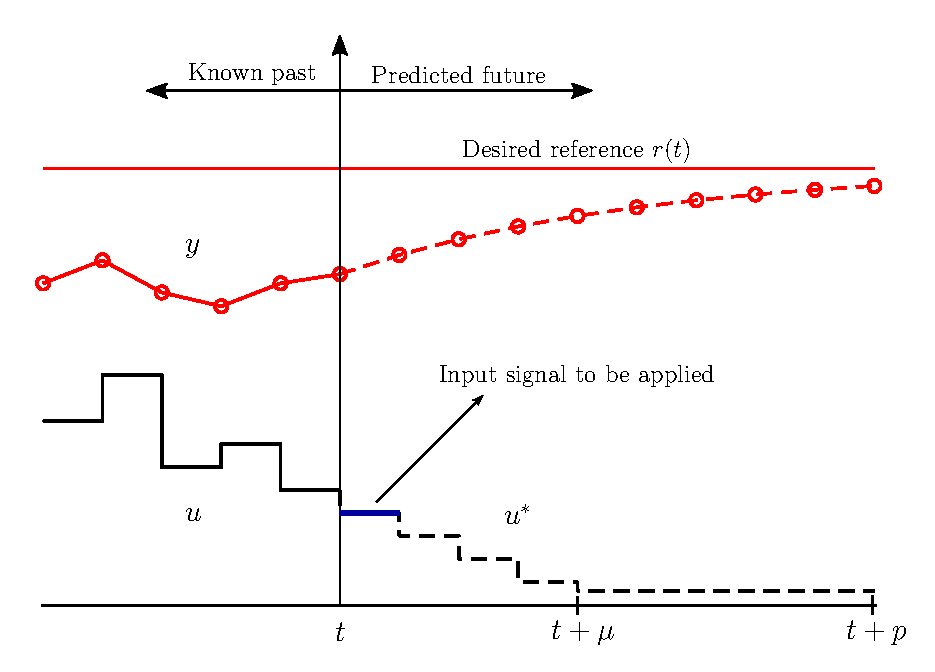
\includegraphics[width = 0.95\textwidth]{Chapter2_SysIDandControl/MPCoverview.pdf}
\caption{A visual example of the MPC optimization problem at sample time $t$. The optimal input sequence is restricted to a move horizon, $\mu$, and the corresponding model-predicted output is also shown.}
\label{fig:MPCoverview}
\end{figure}

\subsection{MPC stability}

Stability is a crucial property in control system design. Generically, and assuming a constant reference $r(t) = r$, a stable control system is one in which the output can be \emph{guaranteed} to remain bounded for all time. For a complete definition of stability, there are sometimes more subtle considerations to be made, for example the internal states of the system should also remain bounded, as well as the control input.

In the earliest days of MPC implementation, the stability of the algorithms was not well understood. While there is certainly a strong relationship between MPC and the more classical feedback control concepts of infinite horizon control and dynamic programming, the now finite horizon and input/state constraints add to the complexity of theoretical analysis \cite{Mayne2000}.

For the simplest case of unconstrained linear MPC, it is sometimes possible to construct an explicit feedback control law from the receding horizon optimization in (\ref{eqn:GeneralMPCOpt}). Thus, stability can be assessed in the same way as for traditional feedback control, by performing an eigenvalue analysis of the linear dynamic state equation in (\ref{eqn:GeneralStateEqn}). For all other cases, stability arguments can be made using the \emph{optimal value function},
\begin{equation}
V_p \big( x(0) \big) = \underset{u(\cdot)}{\text{min }} \sum_{t=1}^{p} \ell(y(t)|x(0),u(t),r(t)). \label{eqn:GeneralOptValue}
\end{equation}
One common approach is to prove that, $\forall x(0) \in \mathcal{X}$, the optimal value function monotonically decreases with each iteration. The receding horizon nature of the problem implies that it is sufficient to show the decrease in any one iteration, i.e.
\begin{equation}
V_p \big( f(x(0),u^*(1)) \big) \leq V_p \big( x(0) \big).
\end{equation}
If such a condition is satisfied, and the penalty function $\ell(y(t),u(t),r(t))$ is positive definite and equal to zero only at the desired input/output setpoint, then stability can be easily shown \cite{Mayne2000},\cite{Grune2011}.

\section{Summary}

Some fundamental concepts in system identification and control were presented in this chapter. The notion of a dynamical system was introduced, and the various stages involved in identifying such systems were discussed. Particular focus was given to the nonparametric impulse response model, which is used to motivate the advantages and drawbacks of common estimation methods such as least squares and maximum likelihood. Some popular regularization techniques were described, with an extensive coverage of quadratically penalized least squares as seen from a Bayesian perspective, which will feature prominently throughout the thesis. Finally, a generic model predictive control formulation was outlined for use in the final part of this thesis.

Many of the concepts introduced in this chapter will be extended in Chapter \ref{chap:3}, where the linear impulse response model is generalized to higher dimensions to produce the Volterra series model. In particular, a method for extending the Bayesian regularization method to Volterra series terms will be explained.